\documentclass{ULBreport} % Llama a tu plantilla adaptada

% Configuración de enlaces (esto sí se queda en el main o se puede mover al .cls)
\hypersetup{
    colorlinks=true,
    linkcolor=black,
    filecolor=magenta,      
    urlcolor=blue,
    citecolor=black,
}

\begin{document}

% 1. GENERAR LA PORTADA CON EL COMANDO ESTRUCTURADO
\titleUCLM{
    title={Valorant Performance Evaluation \\ Un sistema de Inteligencia Artificial para la evaluación objetiva del rendimiento individual en competiciones de esports},
    course={Desarrollo e Integración de Servicios de IA},
    author={{\large Nicolás Celis Moreno}\\[0.7em]
            {\large Erick Mesias Rosero Lesano}\\[0.7em]
            {\large Johann Ismael Ordoñez Echeverría}\\[0.7em]},
    teacher={Julio Alberto López},
    date={2026},
    logoL={Logo_UCLM_40.jpg},
    logoR={esi.png},
    watermark={uclm_fondo.png}
}

% 2. ÍNDICES (Se generan con cuadro gris automáticamente al usar la clase report)
\tableofcontents
\listoftables
\listoffigures


% 3. CONTENIDO PRINCIPAL
% -----------------------------------------------------------------
% NOTA: Usamos \chapter para que el paquete fncychap dibuje el cuadro gris
\chapter{Definición del problema y determinación del alcance}

En este capítulo se detalla la definición del problema seleccionado para la evaluación del proyecto de la asignatura Desarrollo e Integración de Servicios de IA, así como la determinación de su alcance.

\section{Contexto y definición del problema}

En el ecosistema competitivo de Valorant, los equipos que participan en las Valorant Challengers Leagues (VCL) representan el nivel Tier 2 del circuito profesional, funcionando como segunda división o cantera del sistema VCT. Estas organizaciones operan en un entorno altamente competitivo, con presupuestos limitados y márgenes estratégicos reducidos, donde cada decisión relacionada con fichajes, renovaciones o promociones internas tiene implicaciones deportivas, organizativas y económicas significativas.

Más allá del impacto financiero, uno de los principales desafíos que enfrentan estas organizaciones es la evaluación objetiva del rendimiento individual en un juego cuya naturaleza es profundamente contextual y multidimensional. A diferencia de métricas tradicionales basadas únicamente en resultados visibles como asesinatos, daño total o puntuaciones agregadas el desempeño en Valorant depende de variables que interactúan de forma compleja: el rol desempeñado (Duelist, Controller, Sentinel o Initiator), el agente seleccionado, el mapa disputado, la economía del equipo, la gestión de utilidades y la influencia en rondas críticas.

En la práctica, los procesos actuales de análisis en equipos Tier 2 combinan revisión manual de partidas (VOD review), interpretación subjetiva del cuerpo técnico y consulta de estadísticas públicas como K/D, ACS o ADR. Aunque estos métodos aportan información relevante, presentan limitaciones estructurales. El análisis manual es costoso en tiempo y depende de la experiencia del analista; las métricas agregadas tienden a favorecer perfiles orientados al enfrentamiento directo (fraggers o duelists); y la comparación entre jugadores de roles distintos suele realizarse sin una normalización contextual adecuada.

Esta situación genera un margen de error estimado entre el 30\% y el 45\% en decisiones relacionadas con evaluación individual, debido a sesgos cognitivos que priorizan acciones visibles y subestiman contribuciones menos evidentes, como el uso eficiente de utilidades, la creación de espacio, la presión estratégica o la consistencia táctica dentro del rol asignado. En consecuencia, las organizaciones pueden sobrevalorar determinados perfiles y subestimar otros cuya aportación es crítica para la estructura colectiva del equipo.

El problema que se aborda en este proyecto no se limita a generar un ranking general de jugadores, sino a diseñar un sistema de inteligencia artificial capaz de evaluar el desempeño individual dentro del rol específico que ocupa cada jugador, considerando el contexto competitivo en el que se produce dicho rendimiento. El sistema debe aprender la importancia relativa de múltiples métricas técnicas y estratégicas, integrando información procedente de distintas fuentes estructuradas, con el objetivo de producir rankings diferenciados por rol que sean coherentes, explicables y alineados con el análisis experto.

Desde un punto de vista formal, el problema se plantea como un modelo de optimización orientado a ranking, donde cada jugador es representado por un conjunto de variables cuantitativas contextualizadas por agente, mapa y arma. El sistema debe determinar una combinación ponderada de estas variables que permita ordenar a los jugadores de forma consistente, reduciendo el sesgo hacia métricas superficiales y proporcionando una herramienta de apoyo a la decisión para organizaciones Tier 2.

El sistema no pretende reemplazar el criterio humano, sino estructurarlo, reducir su variabilidad y complementar el análisis tradicional con un enfoque reproducible y formalizado. En este sentido, el proyecto aborda simultáneamente un problema competitivo de mejorar la calidad del scouting y la evaluación interna y un problema metodológico para formalizar la evaluación del rendimiento en esports como un sistema interpretable y transferible a otros entornos competitivos digitales.

% FIGURA 1.1
\begin{figure}[H]
    \centering
    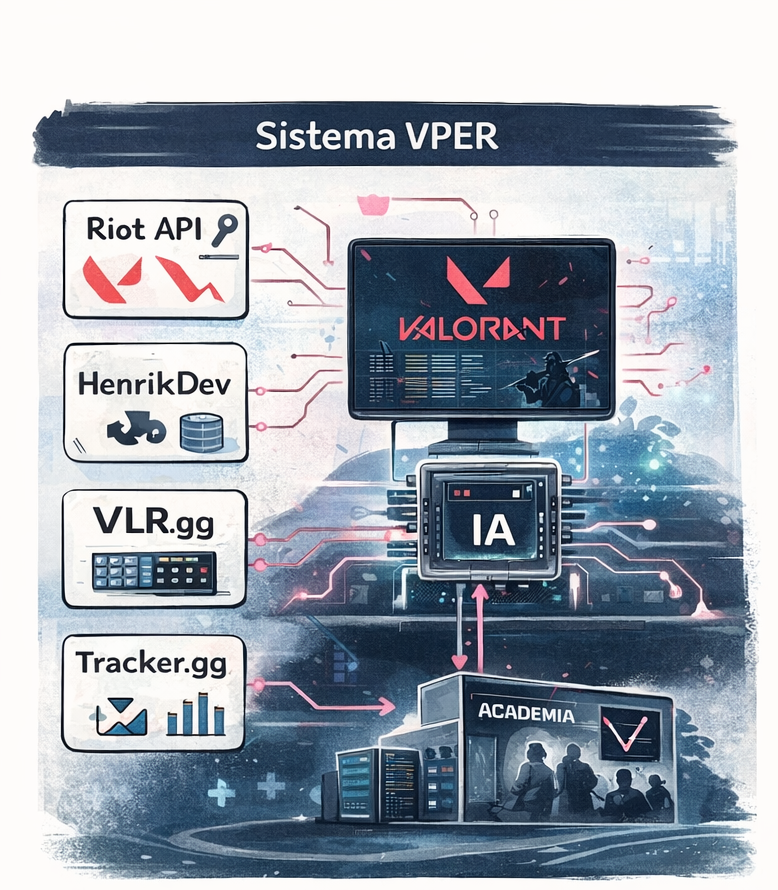
\includegraphics[width=0.9\textwidth]{figura1.png}
    \caption{Arquitectura general del sistema VPER: integración de múltiples fuentes de datos y generación de rankings por rol.}
    \label{fig:arquitectura}
\end{figure}

\section{Objetivos generales y específicos}

El problema que se aborda en este proyecto puede formularse de la siguiente manera:

\textit{¿Cómo diseñar un sistema de inteligencia artificial capaz de evaluar de forma objetiva, consistente y explicable el rendimiento individual de jugadores en un torneo competitivo de Valorant, generando rankings diferenciados por rol?}

Para dar respuesta a esta cuestión, se debe: Diseñar, implementar y validar un sistema de inteligencia artificial capaz de evaluar de forma objetiva, consistente y explicable el rendimiento individual de jugadores en competiciones VCL, generando rankings diferenciados por rol que sirvan como apoyo a decisiones de scouting en equipos Tier 2.

Junto con los objetivos especificos que son los siguientes:

\begin{itemize}
    \item \textbf{Formalizar} el concepto de rendimiento óptimo por rol en Valorant competitivo.
    \item \textbf{Integrar y estructurar} datos históricos procedentes de múltiples APIs públicas.
    \item \textbf{Diseñar} un modelo de optimización orientado a ranking que aprenda pesos contextuales por agente, mapa y arma.
    \item \textbf{Reducir} el sesgo estructural hacia \textit{duelists} y \textit{fraggers}.
    \item \textbf{Evaluar} la coherencia del ranking con valoraciones expertas del staff técnico.
    \item \textbf{Diseñar} el sistema como producto integrable en procesos internos de análisis competitivo.
\end{itemize}

% FIGURA 1.2
\begin{figure}[H]
    \centering
    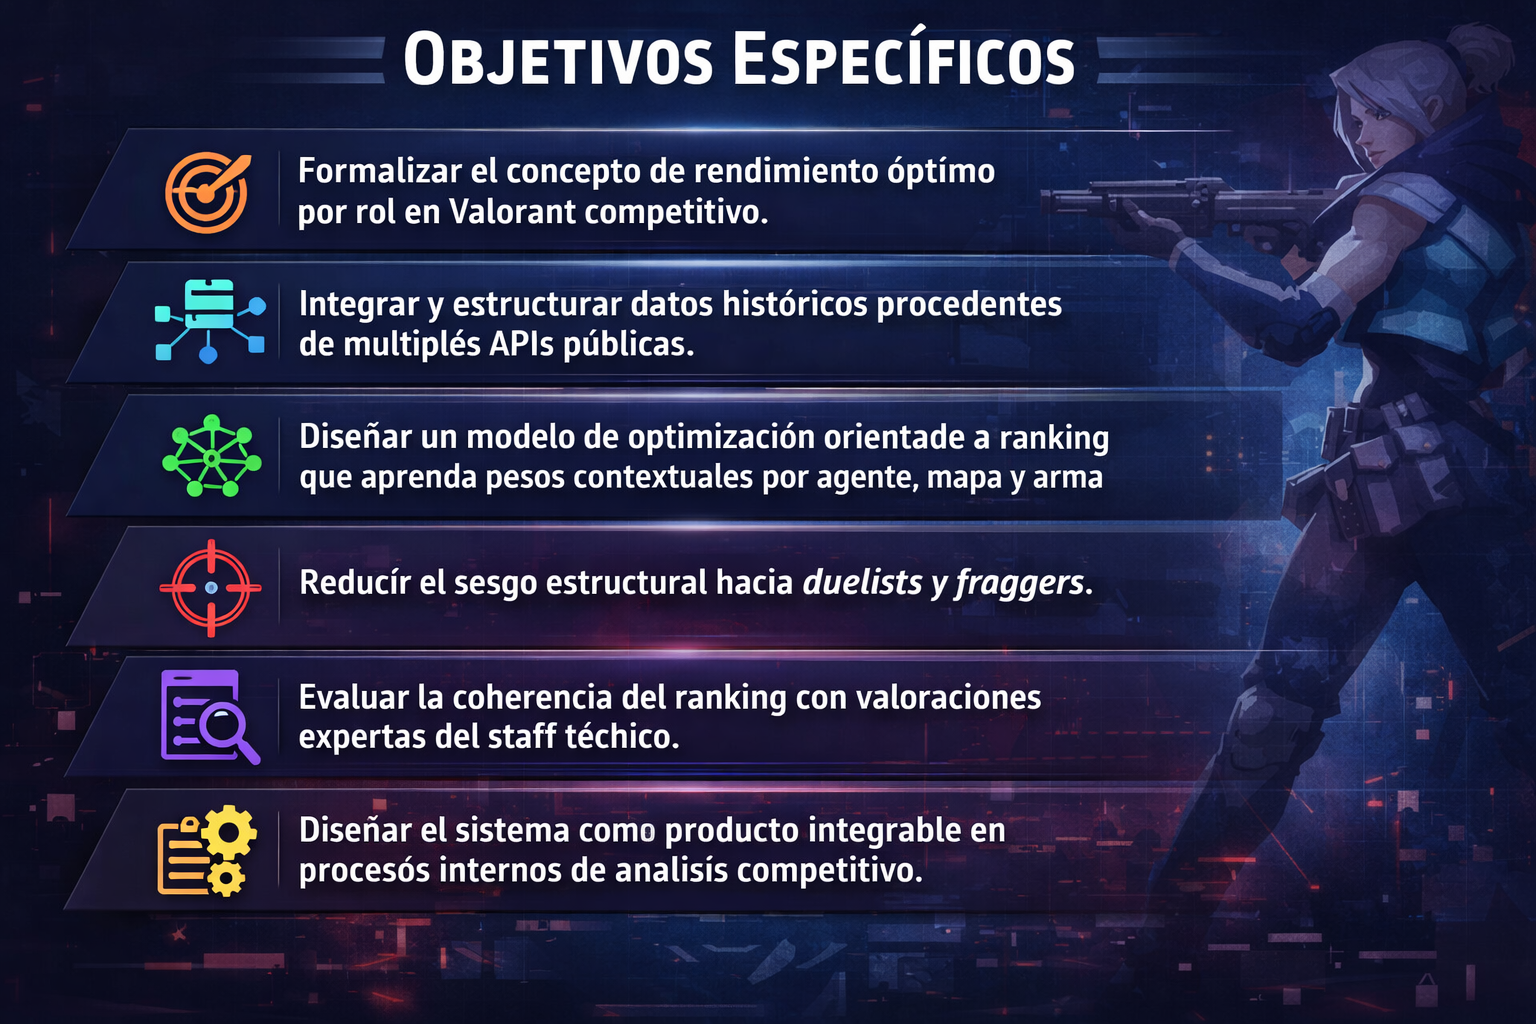
\includegraphics[width=0.8\textwidth]{figura2.png}
    \caption{Objetivos del sistema VPER para la evaluación objetiva del rendimiento en esports.}
    \label{fig:objetivos}
\end{figure}

\section{Determinación del alcance}

El sistema VPER tiene como objetivo delimitar con precisión qué funcionalidades forman parte del proyecto y cuáles quedan explícitamente excluidas, garantizando una ejecución realista dentro del marco temporal de la asignatura y coherente con el desarrollo de un sistema de inteligencia artificial concebido como producto.

El sistema se centrará exclusivamente en la evaluación objetiva del rendimiento individual de jugadores que compiten en torneos pertenecientes a las Valorant Challengers Leagues (VCL), generando rankings diferenciados por rol competitivo (Duelist, Controller, Sentinel e Initiator). Esta delimitación responde a la necesidad de mantener coherencia estructural en la comparación de jugadores, evitando comparaciones transversales entre funciones estratégicamente distintas dentro del juego.

El alcance funcional del proyecto comprende, en primer lugar, la integración de datos históricos estructurados procedentes de múltiples fuentes públicas (Riot API, VLR.gg, Tracker.gg y HenrikDev API). Esta integración no se limita a la mera recopilación de estadísticas agregadas, sino que implica la consolidación, normalización y contextualización de métricas relevantes, tales como rendimiento por agente, impacto por mapa y eficiencia asociada al uso de armas. El objetivo es construir un dataset consistente que permita modelar el desempeño individual desde una perspectiva multidimensional y contextualizada.

En segundo lugar, el sistema incluirá el diseño de un modelo de optimización orientado a ranking, cuya función consistirá en aprender los pesos asociados a cada métrica de rendimiento. Este modelo permitirá generar ordenamientos diferenciados por rol, reduciendo el sesgo estructural hacia métricas centradas exclusivamente en daño o asesinatos, y proporcionando una evaluación más equilibrada del impacto competitivo.

Asimismo, el alcance contempla la evaluación técnica del modelo mediante métricas cuantitativas y la validación cualitativa de los rankings generados a través de su alineación con valoraciones expertas del staff técnico o analistas del dominio competitivo. Esta fase resulta esencial para garantizar que el sistema no se limite a optimizar indicadores estadísticos, sino que produzca resultados interpretables y coherentes con la realidad estratégica del juego.

\subsection{Planificación}

La duración estimada del proyecto es de doce semanas, distribuidas en fases que siguen el ciclo de vida de un proyecto de Machine Learning.

En una primera fase se realizará la definición conceptual del problema, incluyendo la formalización matemática del modelo de ranking y la definición de métricas de evaluación alineadas con el dominio competitivo. Posteriormente, se desarrollará la fase de integración de datos, en la que se implementarán los mecanismos de extracción y consolidación de información procedente de las distintas APIs seleccionadas.

La tercera fase consistirá en el diseño y entrenamiento del modelo de optimización, donde se ajustarán los pesos asociados a cada métrica de rendimiento. A continuación, se llevará a cabo la evaluación técnica del sistema, analizando la coherencia de los rankings generados y su alineación con valoraciones expertas. Finalmente, se desarrollará un prototipo experimental de visualización de resultados que permita demostrar la aplicabilidad práctica del sistema.

Esta planificación garantiza que el proyecto no se limite al entrenamiento de un modelo aislado, sino que abarque todas las etapas necesarias para concebir un sistema de IA como producto funcional.

\subsection{Recursos Humanos: asignación de tareas y capacidad}

El desarrollo del sistema VPER requiere la colaboración de perfiles complementarios que reflejan una estructura realista de proyecto de inteligencia artificial.

El ML Engineer o AI Researcher será responsable de la formulación del problema como modelo de optimización, del diseño de la función objetivo y del entrenamiento del sistema. Este perfil se encargará también del análisis de explicabilidad e interpretación de los pesos aprendidos.

El Data Engineer o Data Analyst asumirá la responsabilidad de integrar las distintas fuentes de datos, desarrollar los procesos de limpieza, normalización y estructuración, y garantizar la consistencia del dataset final. Dado que el sistema depende de múltiples APIs y fuentes externas, este rol resulta crítico para asegurar la calidad del modelo.

El Experto en dominio, en este caso un analista competitivo de Valorant, desempeñará un papel esencial en la validación cualitativa de los rankings generados. Su función será evaluar si los resultados producidos por el sistema son coherentes con la realidad estratégica del juego competitivo.

El stakeholder principal del proyecto será una organización competitiva, academia o equipo semiprofesional de Valorant interesado en mejorar sus procesos de scouting y evaluación de jugadores. El sistema se concibe como herramienta de apoyo a la decisión y no como sustituto del juicio experto.

\subsection{Viabilidad. Estudio del ROI}

La viabilidad económica del sistema VPER se analiza considerando un escenario realista dentro del ecosistema competitivo de Valorant Tier 2 (VCL), donde los equipos operan con presupuestos anuales estimados entre 45.000 y 250.000 dólares, y los salarios promedio por jugador oscilan entre 1.200\,€ y 3.500\,€ mensuales, pudiendo alcanzar los 5.000\,€ en organizaciones con mayor respaldo financiero.

El desarrollo del sistema se estima bajo los siguientes supuestos:

\begin{itemize}
    \item Duración del proyecto: 12 semanas
    \item Equipo de trabajo: 3 personas
    \item Dedicación media: 10 horas semanales por persona
    \item Coste medio estimado por hora: 45\,€
\end{itemize}

Las horas totales invertidas serían:

\[
H = 3 \times 10 \times 12 = 360 \text{ horas}
\]

El coste total estimado del desarrollo sería:

\[
C = 360 \times 45 = 16.200\,€
\]

En el contexto Tier 2, un contrato anual de un jugador puede situarse entre 14.400\,€ y 42.000\,€, dependiendo del nivel competitivo y la región. Un fichaje erróneo no solo implica el coste salarial directo, sino también costes indirectos asociados a bajo rendimiento competitivo, pérdida de oportunidades de clasificación y rotaciones prematuras de plantilla.

Si se considera un escenario conservador en el que el sistema contribuye a evitar un fichaje ineficiente valorado en aproximadamente 20.000\,€ anuales, el retorno de la inversión puede calcularse mediante la fórmula clásica:

\[
ROI = \frac{B - C}{C}
\]

donde $B$ representa el beneficio económico estimado y $C$ el coste de desarrollo.

Sustituyendo valores:

\[
ROI = \frac{20.000 - 16.200}{16.200} \approx 0{,}23
\]

Esto representa un ROI aproximado del 23\% en el primer año de uso.

Este cálculo es deliberadamente prudente y se fundamenta en tres aspectos clave. En primer lugar, el sistema no pretende eliminar completamente el error en la toma de decisiones, sino reducir el margen estimado del 30--45\% asociado al análisis exclusivamente manual. En segundo lugar, el beneficio considerado contempla únicamente el impacto directo de evitar un contrato ineficiente, sin incorporar posibles ahorros en horas de análisis técnico ni la reutilización del sistema en temporadas posteriores. En tercer lugar, el coste de desarrollo es una inversión puntual, mientras que el beneficio puede extenderse en el tiempo mediante su uso recurrente.

Desde esta perspectiva, incluso bajo supuestos conservadores, el sistema VPER presenta viabilidad económica para organizaciones Tier 2, especialmente cuando se considera su potencial de reutilización y mejora continua en ciclos competitivos sucesivos.

\subsection{Valor}

El valor aportado por el sistema VPER se manifiesta en múltiples dimensiones interrelacionadas que trascienden el ámbito puramente técnico.

\begin{description}

    \item[Valor competitivo:] el sistema permite una evaluación objetiva y diferenciada por rol, reduciendo los sesgos tradicionales asociados a métricas superficiales. Esto facilita comparaciones más justas entre jugadores con funciones estratégicas distintas y contribuye a una toma de decisiones más fundamentada.

    \item[Valor organizativo:] el sistema constituye una base tecnológica reutilizable que puede integrarse en procesos internos de scouting, análisis post-partido y planificación estratégica. Al estructurar la evaluación del rendimiento como un modelo formalizado y reproducible, la organización reduce la dependencia exclusiva de valoraciones subjetivas.

    \item[Valor reputacional:] la transparencia en la generación de rankings puede mejorar la credibilidad de decisiones relacionadas con la selección de MVP o fichajes estratégicos. En un entorno altamente mediático como los esports, la percepción de objetividad resulta especialmente relevante.

    \item[Valor tecnológico:] el sistema formaliza la evaluación del rendimiento en esports como un problema de optimización orientado a ranking, integrando múltiples fuentes de datos y manteniendo un enfoque interpretable. Esto sitúa el proyecto no solo como una aplicación práctica, sino como una propuesta metodológica transferible a otros títulos competitivos o disciplinas deportivas digitales.

\end{description}

% -----------------------------------------------------------------
\chapter{Los datos: origen, descripción y análisis}

\section{Introducción}

En este hito se describen y analizan los datos que se utilizarán para abordar el problema planteado en el capítulo anterior, consistente en diseñar, implementar y validar un sistema de inteligencia artificial capaz de evaluar el rendimiento de jugadores profesionales del videojuego competitivo \textit{Valorant}.

El objetivo del sistema es determinar qué jugadores presentan un mayor impacto competitivo dentro de su rol o agente, utilizando métricas de rendimiento extraídas de partidas profesionales. Este sistema pretende servir como herramienta de apoyo para el análisis objetivo del desempeño de los jugadores en competiciones profesionales.

% -----------------------------------------------------------------
\section{Fuentes, origen y tamaño de los datos}

Los datos utilizados para implementar el sistema propuesto provienen de diferentes plataformas que recopilan estadísticas competitivas del videojuego competitivo \textit{Valorant}, incluyendo datos oficiales, APIs públicas y repositorios de análisis de competiciones profesionales. Estas fuentes permiten obtener información detallada sobre el rendimiento individual de los jugadores, así como sobre el contexto de las partidas en torneos profesionales.

Concretamente, el volumen total de datos se obtiene a partir de varias fuentes complementarias que permiten capturar diferentes dimensiones del rendimiento competitivo.

\subsection*{Datos de la API oficial de Riot Games}

La API oficial de Riot Games proporciona acceso a información detallada sobre partidas, jugadores, agentes utilizados y estadísticas de rendimiento dentro del ecosistema competitivo de \textit{Valorant}. A través de esta API es posible obtener datos estructurados sobre el historial de partidas, estadísticas individuales de los jugadores y resultados de los encuentros. Esta fuente constituye una de las principales bases de datos para el análisis del rendimiento competitivo.

\subsection*{Datos de estadísticas competitivas de VLR.gg}

La plataforma VLR.gg recopila información detallada sobre torneos profesionales de \textit{Valorant}, incluyendo estadísticas de jugadores, mapas disputados, equipos participantes y resultados de partidas. Estos datos permiten complementar la información obtenida mediante la API oficial, especialmente en lo relativo al contexto competitivo de los torneos.

\subsection*{Datos de rendimiento de jugadores mediante Tracker Network}

La plataforma Tracker.gg ofrece estadísticas avanzadas sobre el rendimiento de jugadores, tales como métricas agregadas de combate, eficiencia en rondas y análisis histórico de partidas. Estos datos permiten ampliar el conjunto de variables disponibles para el análisis del rendimiento individual.

\subsection*{Datos históricos de competiciones profesionales}

Adicionalmente, se utilizan datasets históricos de resultados y estadísticas de torneos pertenecientes al circuito profesional \textit{Valorant Champions Tour}, así como registros de ligas regionales como la \textit{Challengers League}. Estos datasets incluyen información sobre resultados de partidos, jugadores participantes y estadísticas acumuladas durante los torneos.

Los datos recopilados a partir de estas fuentes se almacenan en formato \texttt{.csv}, lo que permite su tratamiento mediante herramientas de análisis de datos y aprendizaje automático.

\subsection{Estructura del dataset}

En cuanto a la estructura del dataset, los datos presentan una naturaleza tabular. Cada fila del conjunto de datos representa el desempeño de un jugador en una partida o mapa específico dentro de un torneo competitivo. Las columnas contienen las diferentes variables estadísticas asociadas al rendimiento del jugador durante dicha partida.

Entre las variables incluidas en el dataset se encuentran métricas como:

\begin{itemize}
    \item Eliminaciones (\textit{kills})
    \item Muertes (\textit{deaths})
    \item Asistencias (\textit{assists})
    \item Daño promedio por ronda (\textit{ADR})
    \item Puntuación media de combate (\textit{ACS})
    \item Agente utilizado
    \item Mapa de la partida
    \item Economía de rondas y compra de armas
\end{itemize}
\begin{figure}[H]
    \centering
    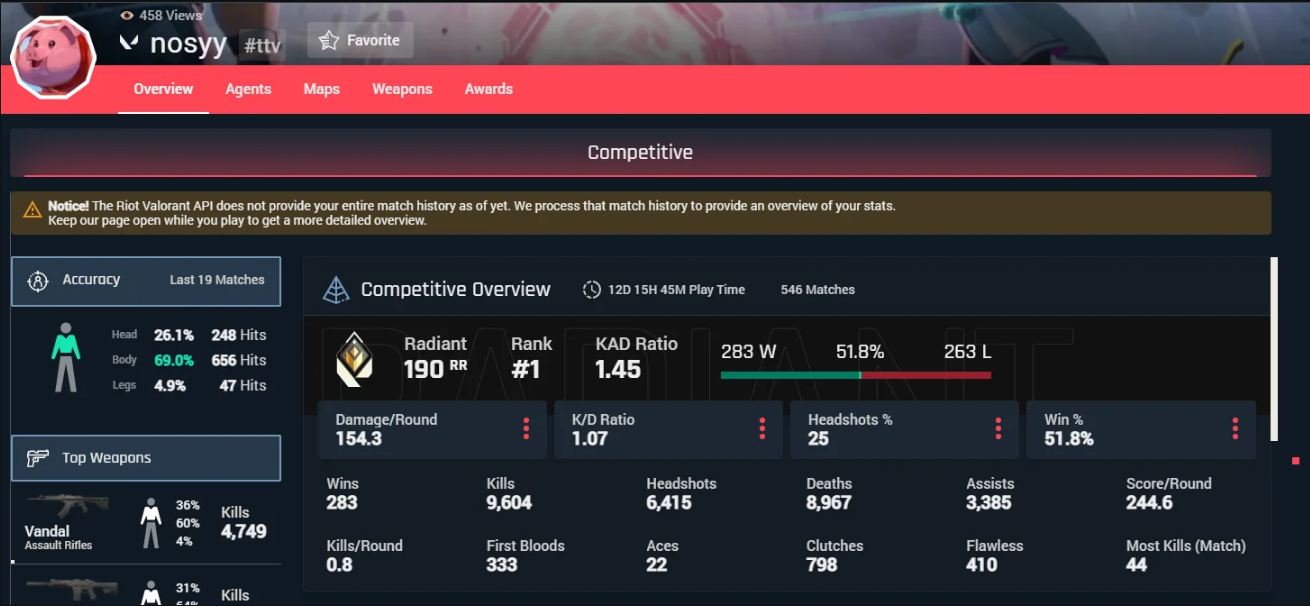
\includegraphics[width=0.95\textwidth]{tracker_stats.png}
    \caption{Ejemplo de panel de estadísticas competitivas de un jugador en la plataforma Tracker.gg.}
    \label{fig:tracker_stats}
\end{figure}
El volumen total de datos recopilados depende de la cantidad de torneos y partidas consideradas en el análisis. De forma aproximada, el dataset final contiene varios miles de registros correspondientes a jugadores en partidas profesionales, con decenas de variables estadísticas por observación que describen diferentes aspectos del rendimiento competitivo.
\section{Inventario de datos}

En esta sección se define el conjunto de datos consolidado con el que trabajará el modelo VPER, tras unificar las distintas fuentes públicas y estructurar la información disponible de los jugadores en las competiciones oficiales.

Tras el proceso de integración, el dataset principal cuenta con más de 50.000 registros correspondientes al rendimiento de jugadores por partida y mapa, estructurado en más de 20 variables cuantitativas clave. Estas métricas engloban tanto la capacidad de eliminación (Kills, First Kills, ACS), como el impacto táctico (Asistencias, Plantado/Desactivado de Spike) y la consistencia en el juego (KAST, ADR).

A continuación, se presenta en la Tabla \ref{tab:inventario_datos} el diccionario con las características seleccionadas que se consideran más representativas a la hora de definir el rendimiento competitivo de un jugador de Valorant.

\begin{table}[H]
    \centering
    \renewcommand{\arraystretch}{1.4}
    \begin{tabular}{@{} l p{0.7\textwidth} @{}}
        \toprule
        \textbf{Variable} & \textbf{Descripción} \\ 
        \midrule
        \textbf{ACS} & Average Combat Score (Puntuación media de combate) \\ 
        \textbf{ADR} & Average Damage per Round (Daño medio por ronda) \\ 
        \textbf{KAST} & \% de rondas con Kill, Assist, Survive o Traded \\ 
        \textbf{First Kills (FK)} & Asesinatos iniciales (Primera sangre de la ronda) \\ 
        \textbf{Assists} & Asistencias totales \\ 
        \textbf{Clutch (1vX)} & Rondas ganadas siendo el último jugador vivo (1v1, 1v2, etc.) \\ 
        \textbf{Spike Plants} & Plantadas de Spike exitosas \\ 
        \textbf{Spike Defuses} & Desactivaciones de Spike exitosas \\ 
        \textbf{Econ Rating} & Daño infligido por cada 1000 créditos invertidos \\ 
        \textbf{Deaths} & Muertes totales por mapa \\ 
        \textbf{First Deaths (FD)} & Muertes iniciales (Primera baja recibida en la ronda) \\ 
        \textbf{Untraded Deaths} & Muertes sin intercambio (el jugador muere y su equipo no logra eliminar al atacante) \\ 
        \textbf{Eco Loss} & Rondas perdidas teniendo superioridad económica \\ 
        \textbf{Spike Defuse Failed} & Rondas perdidas por no lograr desactivar la Spike a tiempo \\ 
        \bottomrule
    \end{tabular}
    \caption{Inventario de datos: diccionario.}
    \label{tab:inventario_datos}
\end{table}

Antes de proceder con el modelado, es fundamental establecer ciertas limitaciones y consideraciones sobre la naturaleza de estos datos en el ecosistema de Valorant:

\begin{itemize}
    \item \textbf{El problema de los jugadores flexibles (Flex players):} En el dataset, algunos jugadores alternan entre posiciones (por ejemplo, juegan \textit{Initiator} en un mapa y \textit{Duelist} en otro). El sistema debe aislar y evaluar el rendimiento del jugador por cada rol específico que desempeña, en lugar de realizar una media global que distorsionaría su perfil.
    \item \textbf{Impacto invisible (Utilidad):} Las APIs públicas presentan limitaciones para capturar el 100\% del impacto táctico. Una habilidad de control (como un muro o un humo) puede ganar una ronda cortando una rotación enemiga, pero no registrarse como asistencia directa. El modelo debe compensar esto infiriendo impacto a través del porcentaje de victorias en el mapa (KAST) y no solo con K/D.
    \item \textbf{Contexto económico:} No todas las bajas tienen el mismo peso. Una baja en una ronda de tipo "Eco" frente a rivales con compra completa ("Full Buy") tiene un impacto táctico y económico mucho mayor que un asesinato de impacto residual al final de una ronda ya perdida.
    \item \textbf{Normalización por rondas (Métricas \textit{Per-Round}):} Dado que la duración de las partidas en Valorant es variable (desde un rápido 13-0 hasta múltiples prórrogas), no es viable utilizar métricas absolutas (como \textit{Total Kills} o \textit{Total Damage}). Todas las variables cuantitativas de volumen deben transformarse a su equivalente por ronda (por ejemplo, KPR - \textit{Kills Per Round}, ADR - \textit{Average Damage Per Round}) para garantizar una comparativa justa e independiente de la duración del partido.
    \item \textbf{El impacto de las actualizaciones (Parches):} El metajuego competitivo está sujeto a actualizaciones periódicas de Riot Games que alteran el balance de los agentes, la economía y el diseño de los mapas. El dataset debe acotar su alcance a un parche específico o normalizar el rendimiento de un agente comparándolo únicamente con la media histórica de ese mismo agente durante esa versión concreta del juego.
\end{itemize}

\section{Análisis de los datos}

El análisis exploratorio de los datos (EDA) se ha llevado a cabo mediante un entorno de procesamiento en Python, estudiando de forma sistemática la estructura, distribución y correlación entre las distintas métricas de rendimiento. En este análisis se han abordado los siguientes aspectos fundamentales:

\begin{itemize}
    \item Distribución estadística de métricas de impacto directo (ACS, ADR, Kills) frente a métricas de impacto táctico (KAST, Asistencias, Spike Plants).
    \item \textbf{Multicolinealidad entre métricas de impacto:} El análisis revela una altísima correlación lineal entre variables de daño y eliminación, particularmente entre el ACS (\textit{Average Combat Score}) y el ADR (\textit{Average Damage per Round}). El modelo de IA deberá tratar esta redundancia para evitar sobreponderar el daño bruto en detrimento del impacto táctico.
    \item \textbf{Sesgo de los mapas (\textit{Map Skew}):} A partir de las estadísticas globales, se identifica que ciertos mapas presentan un fuerte desbalance hacia uno de los bandos (por ejemplo, mapas marcadamente \textit{Defender-sided}). Este hallazgo sugiere que el modelo debería considerar un factor de corrección contextual: conseguir una Primera Sangre (\textit{First Kill}) en el lado atacante de un mapa favorable a la defensa aporta un valor marginal mayor a la victoria que lograrla en el lado favorable.
    \item Estudio del perfil estadístico agrupado por rol competitivo (Duelist, Controller, Sentinel, Initiator) e identificación de valores atípicos en partidas con prórrogas (\textit{Overtime}).
\end{itemize}

Los resultados de este análisis exploratorio confirman que las variables de rendimiento en Valorant presentan distribuciones fuertemente asimétricas y altamente dependientes del rol desempeñado. Por ejemplo, métricas como los First Kills (FK) o el ACS muestran picos de concentración pronunciados en los jugadores que asumen el rol de Duelist, mientras que las Asistencias o el KAST dominan el perfil estadístico de los Initiators y Controllers.

Esta heterogeneidad estructural justifica la decisión de diseño central del sistema VPER: la evaluación de rendimiento no puede realizarse mediante un ranking global absoluto, sino que requiere generar rankings diferenciados e independientes para cada demarcación estratégica del juego.

\section{Evaluación del rendimiento. Métricas}

Una vez analizada la estructura de los datos, es necesario definir matemáticamente cómo el sistema va a evaluar el rendimiento para generar los rankings de jugadores en cada rol.

Aunque la base de datos recoge si un jugador ha sido destacado por expertos o ha formado parte del equipo ideal de un torneo, el problema no debe plantearse como una simple clasificación binaria (predecir si será destacado o no). El objetivo es construir un ranking ordenado. Para ello, se define el rendimiento o \textit{scoring} de un jugador mediante una combinación ponderada de las características de su juego, tal y como se muestra en la Ecuación \ref{eq:scoring}.

\begin{equation}
    \text{scoring}(p) = \sum_{i=1}^{n} x_{i} \cdot w_{i}
    \label{eq:scoring}
\end{equation}

Donde:
\begin{itemize}
    \item $p$: Es un jugador del torneo evaluado en un rol específico.
    \item $x_{i}$: Es el valor de la métrica estadística $i$ (por ejemplo, ADR, Asistencias, First Kills) obtenida del dataset.
    \item $w_{i}$: Es el peso o la contribución de la métrica $i$ al rendimiento total del jugador.
\end{itemize}

No todas las acciones tienen el mismo impacto en el rendimiento de un jugador. Algunas acciones contribuyen positivamente a la puntuación del jugador (sumando valor), mientras que otras contribuyen negativamente (penalizando). Las Tablas \ref{tab:variables_positivas} y \ref{tab:variables_negativas} muestran las variables del dataset diferenciadas por su aporte positivo o negativo al \textit{scoring} del jugador.

\begin{table}[H]
    \centering
    \renewcommand{\arraystretch}{1.4}
    \begin{tabular}{@{} l p{0.65\textwidth} @{}}
        \toprule
        \textbf{Variables Positivas} & \textbf{Significado} \\ 
        \midrule
        \textbf{ACS} & Average Combat Score (Puntuación media de combate) \\ 
        \textbf{ADR} & Average Damage per Round (Daño medio por ronda) \\ 
        \textbf{KAST} & \% de rondas con Kill, Assist, Survive o Traded \\ 
        \textbf{First Kills (FK)} & Asesinatos iniciales (Primera sangre de la ronda) \\ 
        \textbf{Assists} & Asistencias totales \\ 
        \textbf{Clutch (1vX)} & Rondas ganadas siendo el último jugador vivo (1v1, 1v2, etc.) \\ 
        \textbf{Spike Plants} & Plantadas de Spike exitosas \\ 
        \textbf{Spike Defuses} & Desactivaciones de Spike exitosas \\ 
        \textbf{Econ Rating} & Daño infligido por cada 1000 créditos invertidos \\ 
        \bottomrule
    \end{tabular}
    \caption{Diccionario de variables separando características con impacto positivo.}
    \label{tab:variables_positivas}
\end{table}

\begin{table}[H]
    \centering
    \renewcommand{\arraystretch}{1.4}
    \begin{tabular}{@{} l p{0.65\textwidth} @{}}
        \toprule
        \textbf{Variables Negativas} & \textbf{Significado} \\ 
        \midrule
        \textbf{Deaths} & Muertes totales por mapa \\ 
        \textbf{First Deaths (FD)} & Muertes iniciales (Primera baja recibida en la ronda) \\ 
        \textbf{Untraded Deaths} & Muertes sin intercambio (el jugador muere y su equipo no logra eliminar al atacante) \\ 
        \textbf{Eco Loss} & Rondas perdidas teniendo superioridad económica \\ 
        \textbf{Spike Defuse Failed} & Rondas perdidas por no lograr desactivar la Spike a tiempo \\ 
        \bottomrule
    \end{tabular}
    \caption{Diccionario de variables separando características con impacto negativo.}
    \label{tab:variables_negativas}
\end{table}

Para asegurar la explicabilidad del modelo y su coherencia con la teoría del juego competitivo, el dominio de los pesos no es infinito ni aleatorio. Se establece un rango estandarizado $[-2, 2]$ para representar el dominio de las variables de decisión. Específicamente, para garantizar la coherencia semántica, el dominio de las variables con impacto positivo pertenecerá al intervalo $[(0+\mu), 2]$ y el de las variables negativas al intervalo $[-2, -(0+\mu)]$, siendo $\mu$ un umbral mínimo mayor que cero. 

Esta restricción de diseño garantiza que una acción perjudicial jamás pueda sumar puntuación a un jugador, y una acción beneficiosa jamás pueda restarla. De este modo, la interpretación del ranking resultante se mantiene estrictamente alineada con la lógica táctica de Valorant.

A partir de las puntuaciones calculadas, es posible obtener una clasificación o ranking ordenando las puntuaciones de los jugadores de acuerdo a la Ecuación \ref{eq:ranking}.

\begin{equation}
    \text{ranking} = \text{sort}(\text{scoring}(p)) \quad \forall p \in P
    \label{eq:ranking}
\end{equation}

siendo $P$ el conjunto de todos los jugadores que han competido en dicho rol.

En estudios previos de analítica deportiva se ha utilizado frecuentemente la media del rango recíproco (en inglés \textit{Mean Reciprocal Rank}, MRR) como función objetivo, tal y como se muestra en la Ecuación \ref{eq:mrr}.

\begin{equation}
    \text{MRR}(\text{ranking}) = \frac{1}{N} \sum_{i=1}^{N} \frac{1}{\text{rank}_{\text{best}}}
    \label{eq:mrr}
\end{equation}

donde $N$ es el número de veces que se construye la clasificación o el número de repeticiones del experimento, y $\text{rank}_{\text{best}}$ es la posición ocupada en la clasificación por el mejor jugador real. Esta métrica permite determinar un conjunto de pesos con el fin de crear una clasificación en la que el mejor jugador ocupe el primer lugar. Sin embargo, esta métrica sigue un enfoque ciego, ya que las ponderaciones se ajustan teniendo en cuenta solo al primer clasificado, lo que ofrece resultados que a nivel competitivo generan sobreajuste y no reflejan la profundidad del rendimiento general.

Para solucionar estos problemas, en este sistema se introduce la métrica de Precisión Media en Promedio (MAP). A diferencia de la métrica MRR, MAP ajusta los pesos para obtener una clasificación en la que el objetivo es encontrar el mayor número posible de jugadores destacados y garantizar que ocupen las posiciones más altas del ranking. Su definición matemática viene dada por la Ecuación \ref{eq:map}.

\begin{equation}
    \text{MAP}(\text{ranking}) = \frac{1}{N} \sum_{i=1}^{k} \frac{i}{\text{rank}_{i}} \quad \text{si } i \le \text{rank}_{i}
    \label{eq:map}
\end{equation}

Donde $N$ es el número de repeticiones del experimento, $k$ es el número máximo de jugadores del top considerados (por ejemplo, los 5 mejores jugadores del torneo en ese rol) y $\text{rank}_{i}$ es la posición real que el modelo ha otorgado al jugador $i$. MAP es una función acotada entre 0 y 1. Dado el volumen de datos disponible, debe prestarse especial atención al riesgo de sobreajuste (\textit{overfitting}) en el proceso de optimización de pesos, motivo por el cual MAP resulta mucho más robusta que MRR.

De esta manera, se plantea el siguiente problema de optimización central del proyecto: dados los valores estadísticos de cada jugador, el objetivo del sistema de Inteligencia Artificial es encontrar la combinación de pesos ($w$) que maximice el valor de la métrica MAP, logrando que el ranking generado coincida lo máximo posible con el criterio de los expertos. La Ecuación \ref{eq:max_map} muestra la formulación del problema planteado.

\begin{equation}
    \max_{w} \text{MAP}(\text{ranking})
    \label{eq:max_map}
\end{equation}

Las variables de decisión del problema son los pesos asociados a cada estadística. Este problema se resolverá de forma independiente cuatro veces, una por cada rol del juego (Duelist, Controller, Sentinel e Initiator), obteniendo así un modelo de evaluación específico y contextualizado para cada demarcación de la pista.

% =================================================================
% BIBLIOGRAFÍA (Añadir fuentes bibliográficas)
% =================================================================
\newpage
\begin{thebibliography}{9}

    \bibitem{Dex23}
    Gonzalez, M. (2023). 
    \textit{How much do Valorant pros make? Salaries, prize money and earnings explained}. 
    Dexerto Esports News.

    \bibitem{Esp24}
    Brown, T. (2024). 
    \textit{Valorant player salaries: How much do VCT pros earn?}. 
    Esports.net.

    \bibitem{Dot22}
    Scott, R. (2022). 
    \textit{Average salaries in Valorant esports and how contracts work}. 
    Dot Esports.

    \bibitem{Earn25}
    Esports Earnings. (2025). 
    \textit{Top earning Valorant players and prize money statistics}. 
    EsportsEarnings Database.
    \end{thebibliography}

\end{document}
